\section{Progress}
\label{sec:Progress}

As a preeliminary step in research, we first established a corpus of
the top 75 news and sports websites on which we woudl run most of our
experiments in order to cater to the most popular and compute
intensive websites.  These websites are taken from the Alexa top
website list \cite{}.  We ran all our experiments on Macbook Pro 2017,
Google Pixel 2, and Moto G5 to contrast performance numbers between
the three most famous devices with drastically different compute
powers. We used chrome v 61 to run all  our experiments both on the
desktop and the mobile devices. We leveraged chrome developer tools in
order to capture the runtime traces both for network and compute. We
then analysed these runtime traces to draw insight into the critical
path of the website, the total time being spent on the compute vs the
total time being spent on the network, and most importantly the finer
level breakdown of the computation time to understand the true nature
of computation on mobile devices. 

\begin{figure*}[!bth]
\begin{subfigure}[b]{0.5\textwidth}
\centering
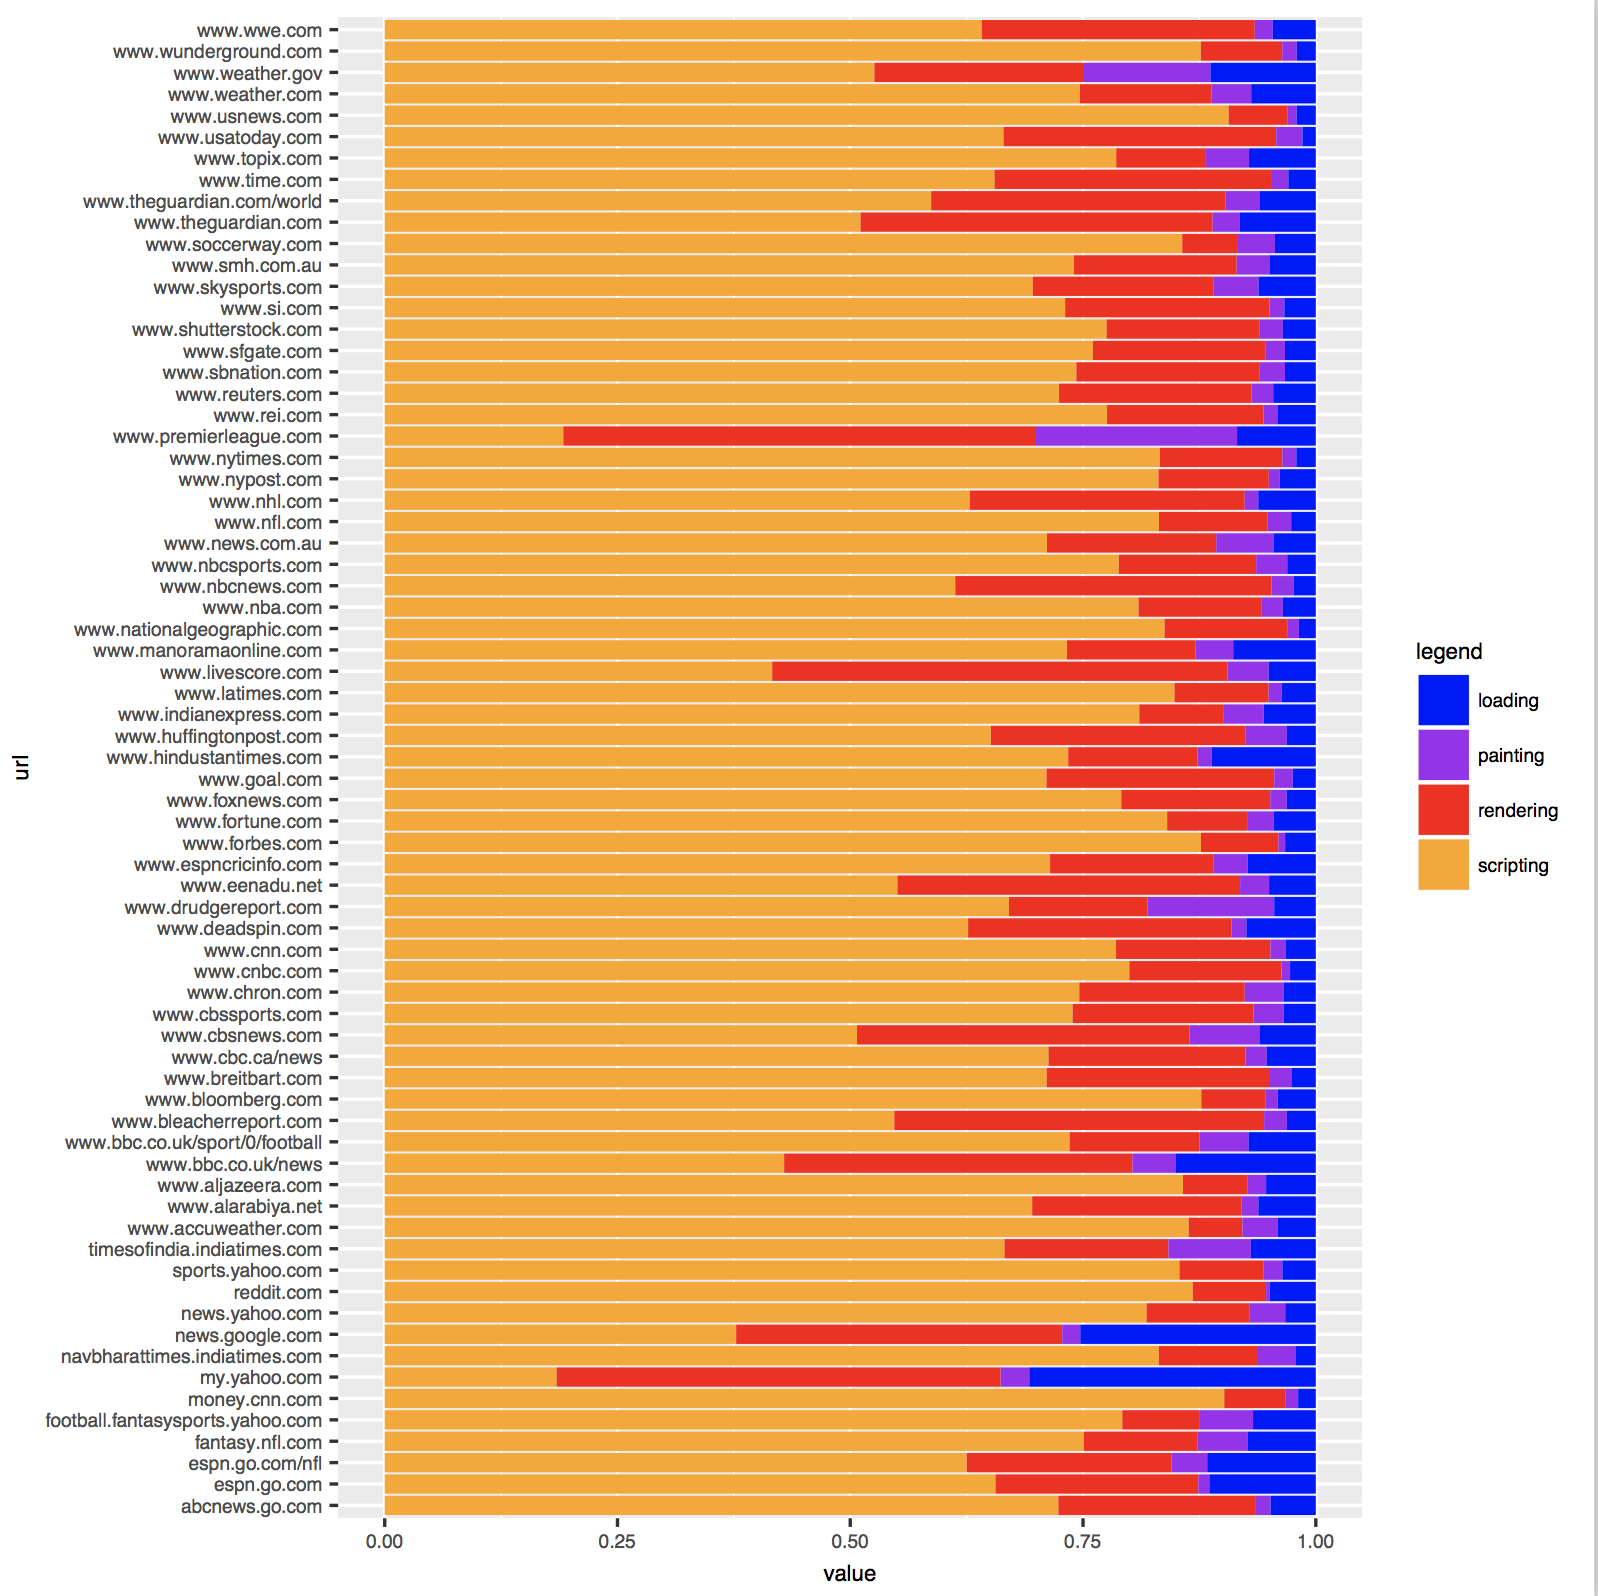
\includegraphics[width=0.9\columnwidth]{figs/cat_p2.png}
\caption{Breakdown of computation on pixel 2}
\label{fig:act_p2}
\end{subfigure}
\begin{subfigure}[b]{0.5\textwidth}
\centering
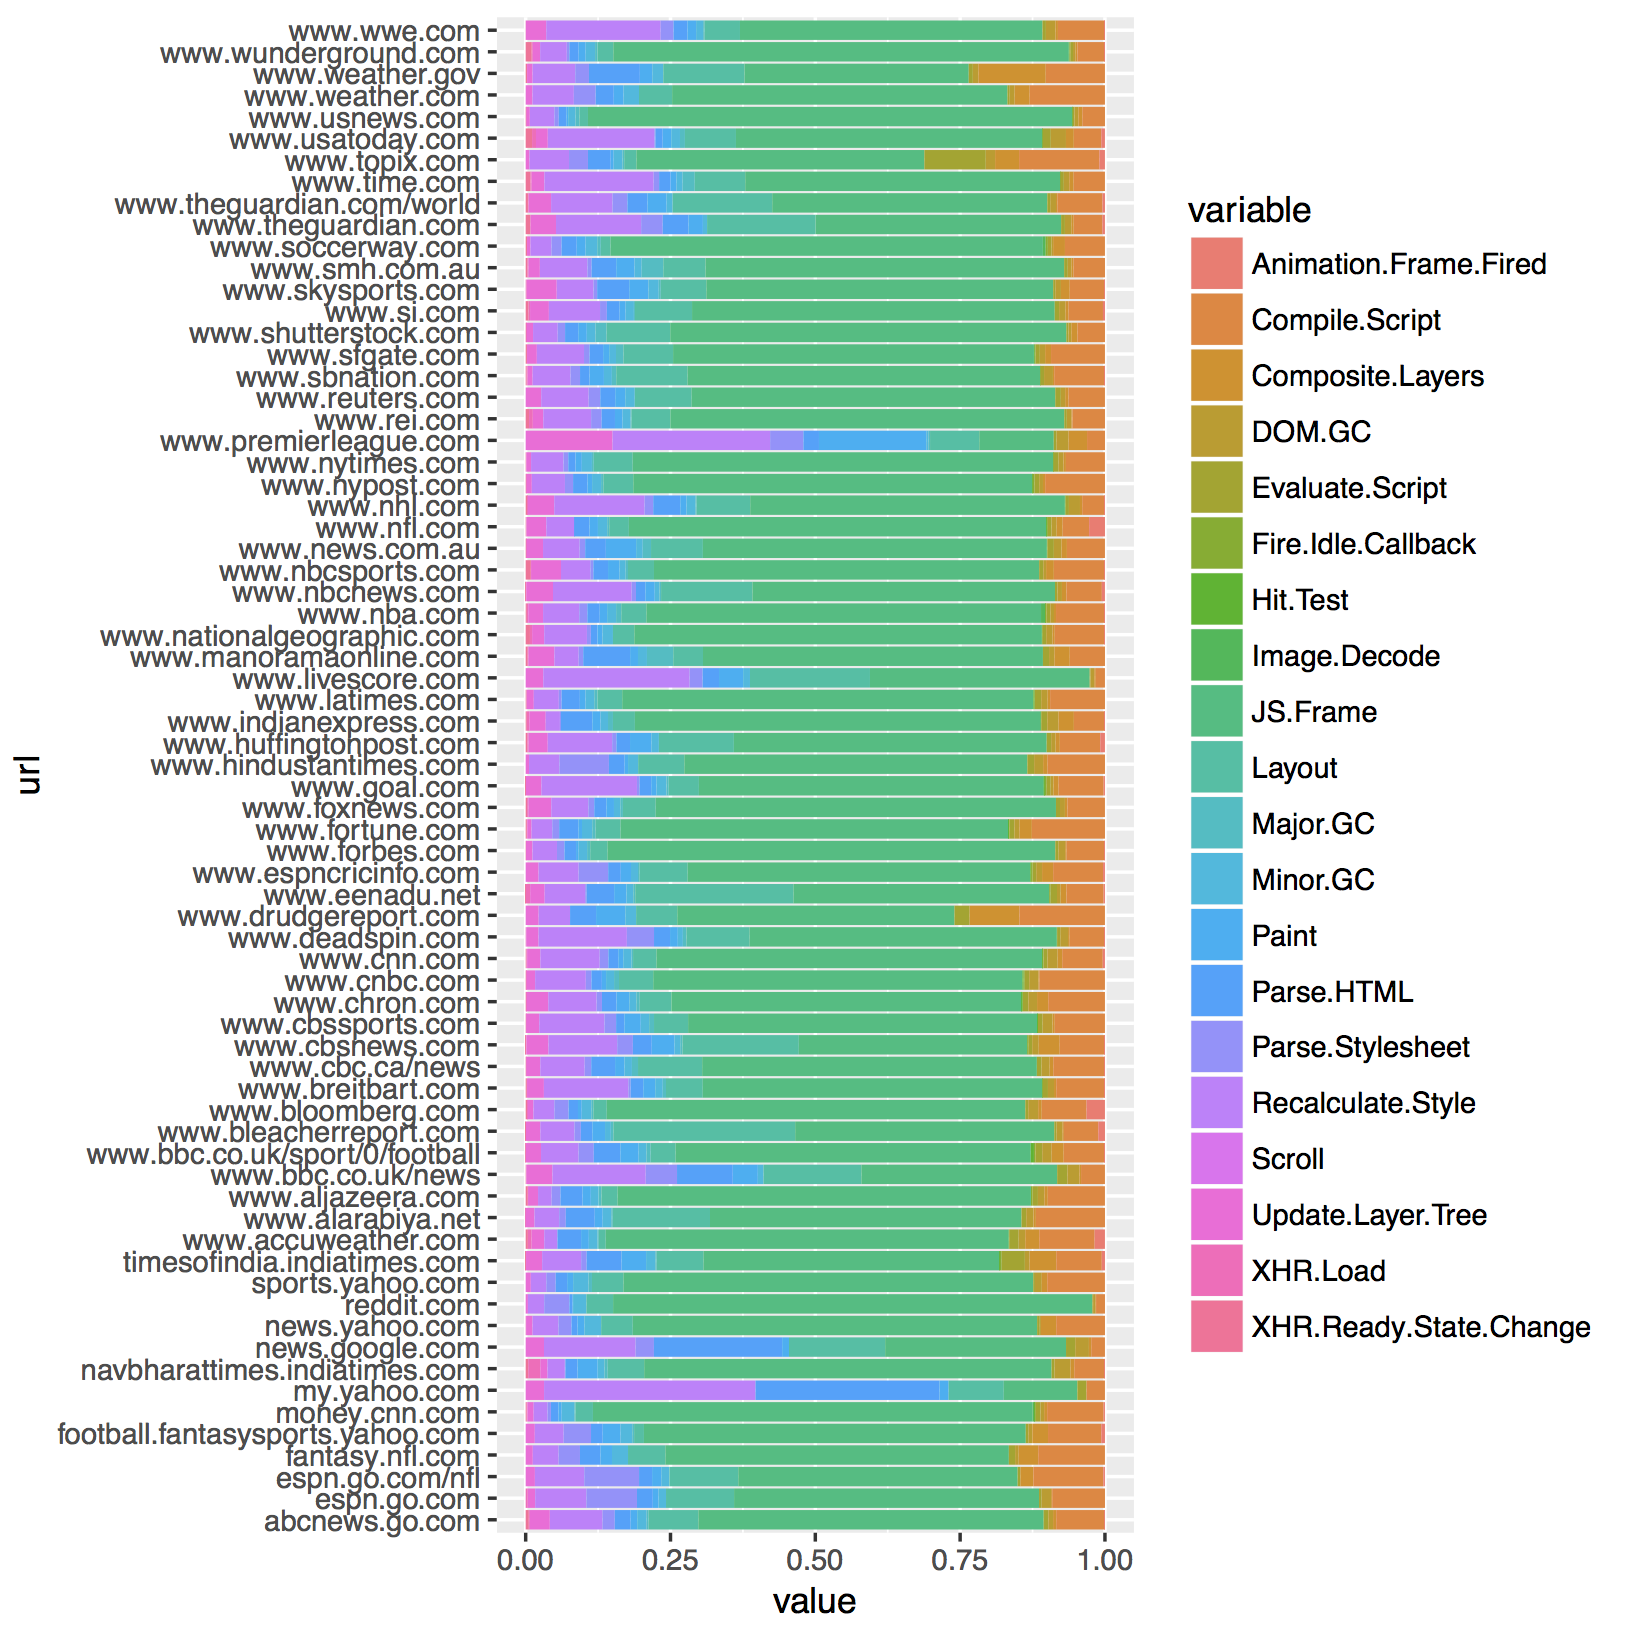
\includegraphics[width=0.9\columnwidth]{figs/act_p2.png}
\caption{Breakdown of computation into finer events on pixel 2}
\label{fig:cat_p2}
\end{subfigure}
\caption{{\color{red}Figure 2 captioon placeholder}}
\end{figure*}
We categorised computation time into four categorires, scripting,
loading, rendering and painting. Scripting is the total time being
spent on compiling javascript, evaluating and executing it. Loading is
the parsing of html and css, which happens immediately after the
payload for the network requests are received by the browser. Loading
essentially takes these payload objects and parses them and converts
them to a DOM tree. Once the DOM tree is built, the rendering engine
kicks in which starts to convert this DOM tree into a render tree,
which contains the exact coordinates and the shape of each of the DOM
node. This is what rendering time comprises of.  Painting time is the
time taken to process the render tree, and actually convert each pixel
into a bitmap.  Figure~\ref{fig:act_p2} shows the computation break
down for these first level of categories for Google pixel 2. We
further break down this time into the most finest level events which
are returned by Google Chrome's trace and then group them by their
event name.

These results are extremely coherent with our design of implementing a
javsvcript chrome caching mechanism and show the possibility of a
large improvement in the total page load due to the high percentage
share of execution time as seen in Figure~\ref{fig:cat_p2}.
\begin{figure*}[!bth]
\begin{subfigure}[b]{0.5\textwidth}
\centering
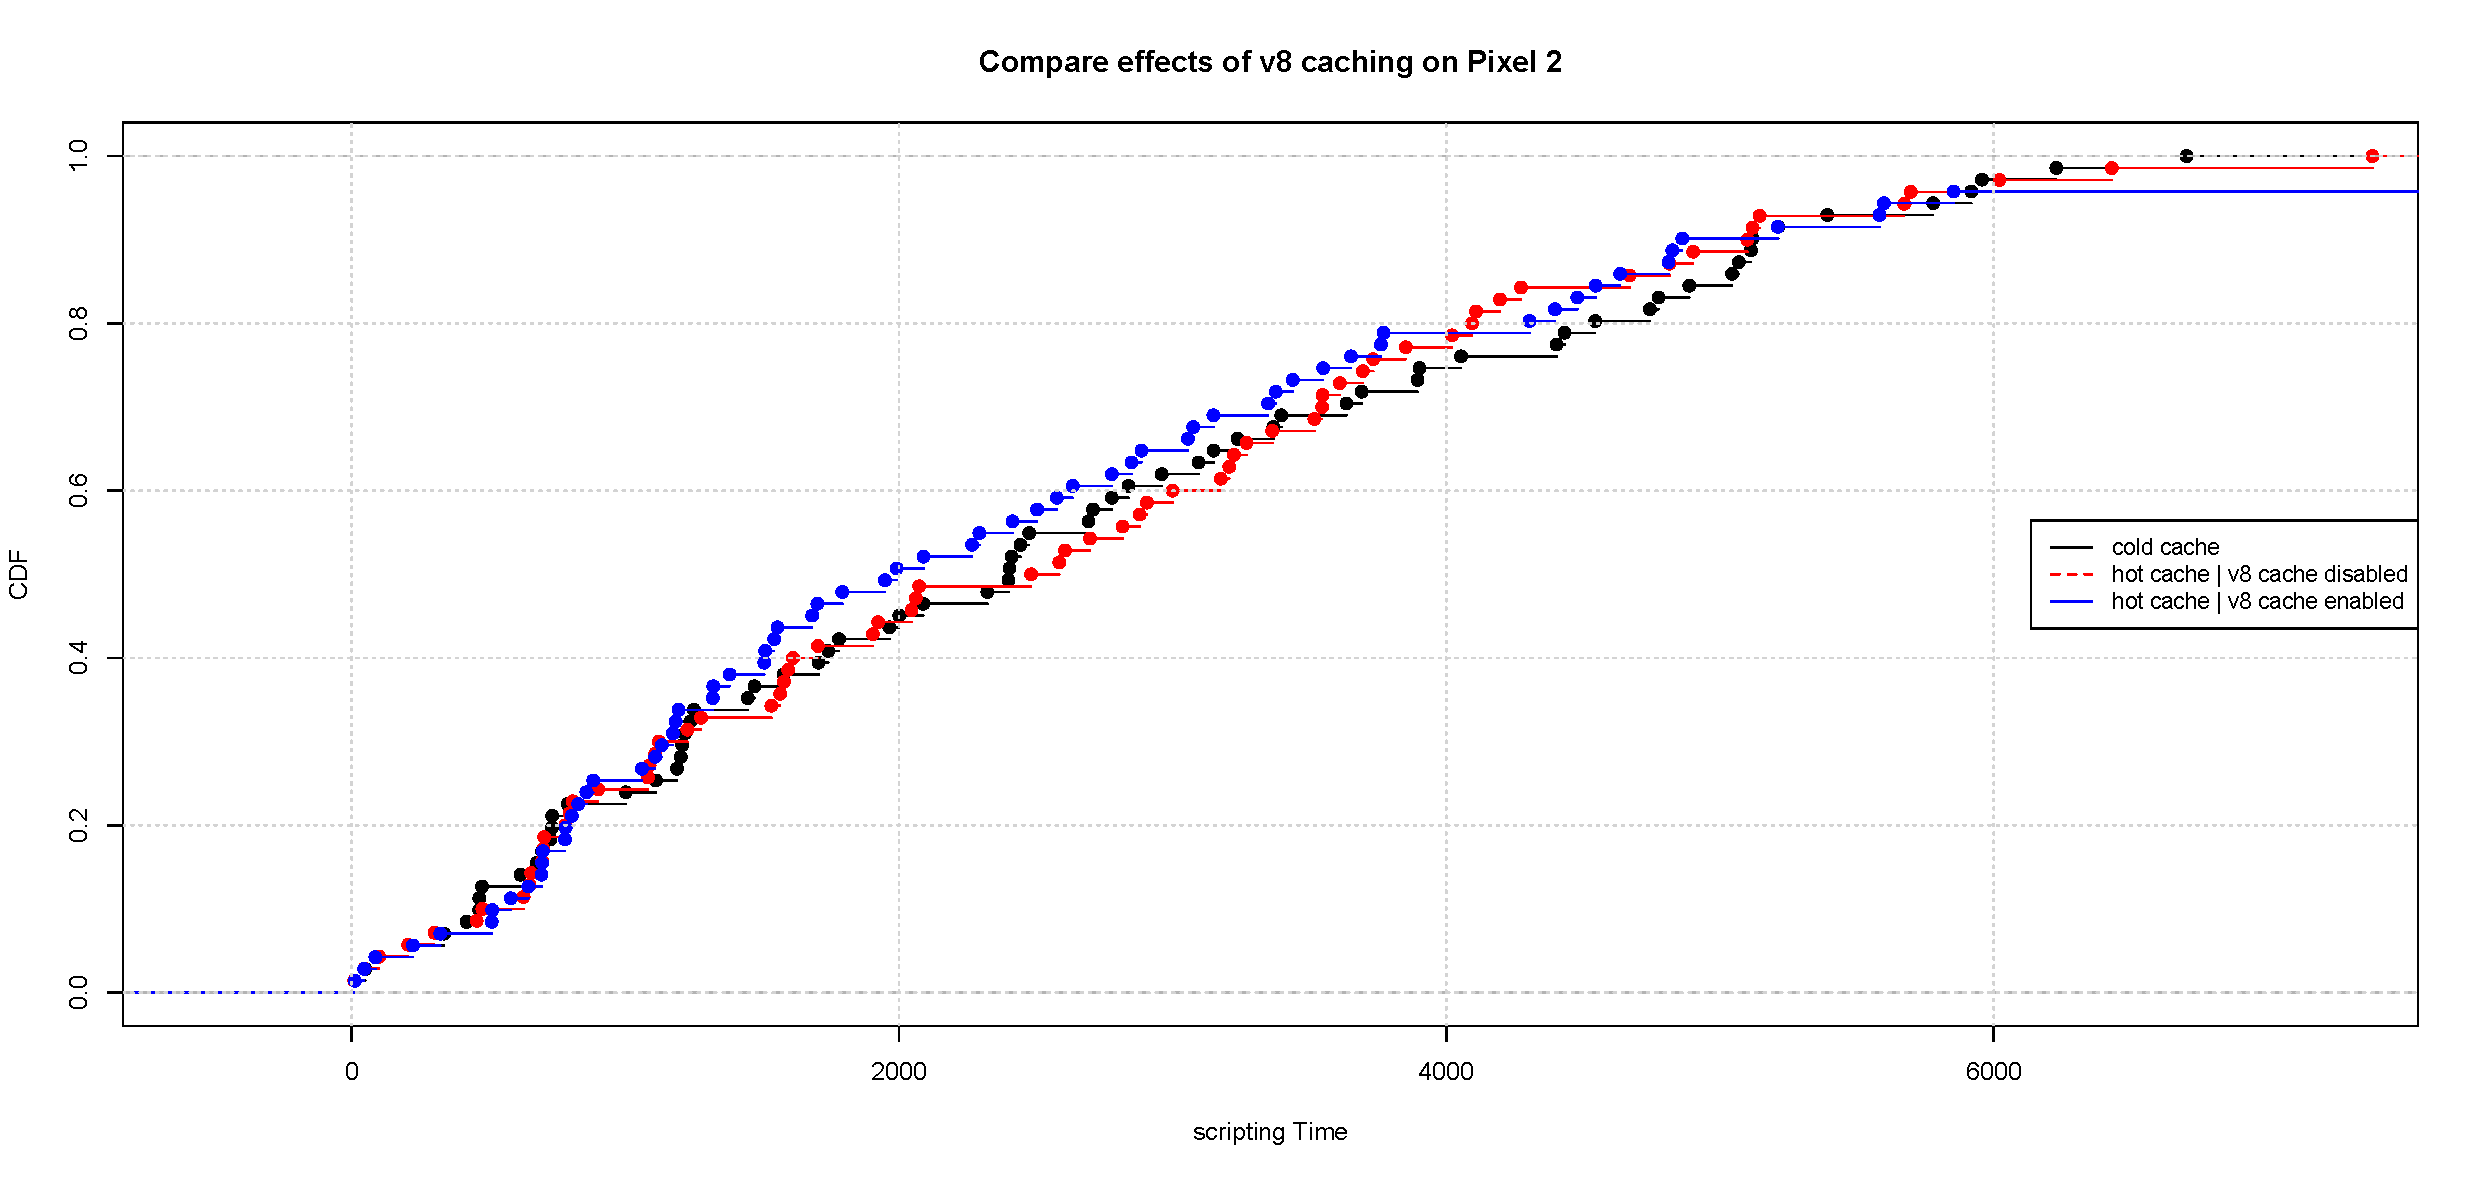
\includegraphics[width=0.9\columnwidth]{figs/v8cache_P2_scripting.pdf}
\caption{Comparison of total scripting time with and without chrome's optimisations}
\label{fig:scripting_p2}
\end{subfigure}
\begin{subfigure}[b]{0.5\textwidth}
\centering
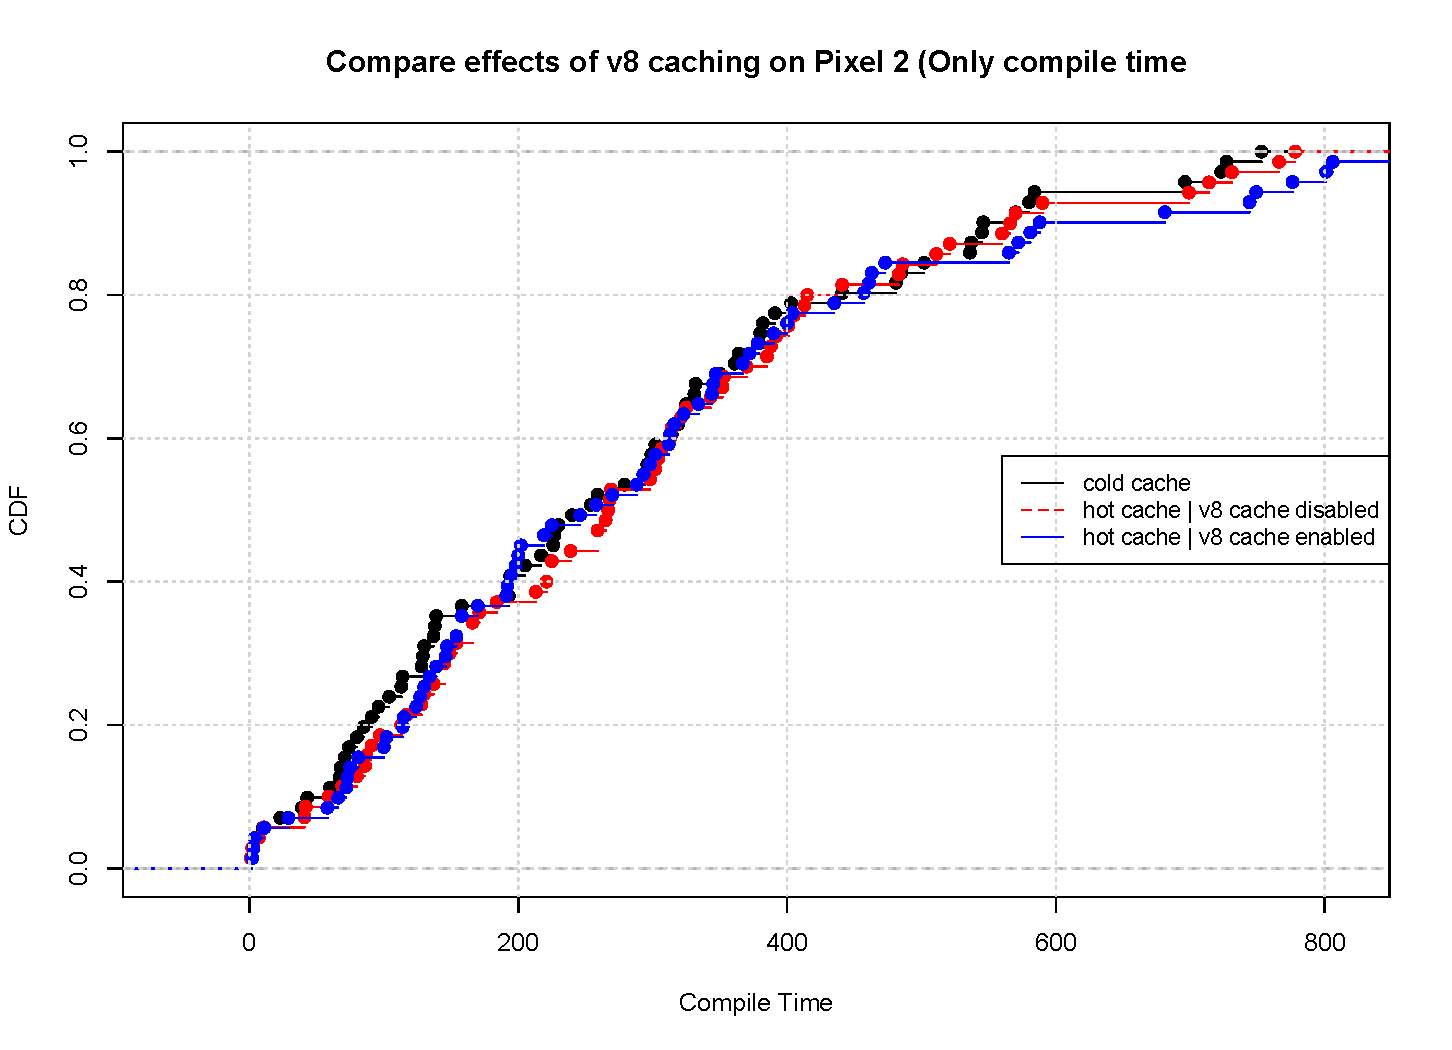
\includegraphics[width=0.9\columnwidth]{figs/v8cache_P2_compile.pdf}
\caption{Comparison of total compiling time with and without chrome's optimisations}
\label{fig:compile_p2}
\end{subfigure}
\caption{{\color{red}Figure 3 captioon placeholder}}
\end{figure*}

Recently Chrome in their 2017 dev summit talked about the various
optimisation techniques they have employed in the latest chrome
browser to improve the total page load time.  We did a comparison of
the total page load with and without chrome's optimisation to see the
improvements. As we can see, there has been a significant reduction in
the overall scripting time. This is primarily due to the introduction
of compiler and parser cache.  We further broke down this computation
and compared the exact compile time across different optimisation
settings. We first captured trace for the top 75 websites with the
chrome compile and parse optimization disabled and then again with the
optimization enabled. As shown in Figure~\ref{fig:compile_p2} to our
suprise, there was no reduction in the compile time, as opposed to the
claim by Chrome quoting a 40\% decrease in the overall compile time.
All of our work will be on top of Chrome's latest changes to ensure
compatibility and relevance of our work. 
